\begin{enumerate}
	\item Write the common difference of the A.P. :$\frac{1}{5}, \frac{4}{5}, \frac{7}{5}, \frac{10}{5}, \cdots$

	\item Find the $8^{th}$ term of the A.P. whose first term is $-2$ and common difference is $3$.
	\item
	Roshini being a plant lover decides to start a nursery. She bought few plants with pots.She placed the pots in such a way that the number of pots in the first row is $2$, in the second is $5$, in the third row is $8$ and so on.
		\begin{figure}[h]
			\centering	
			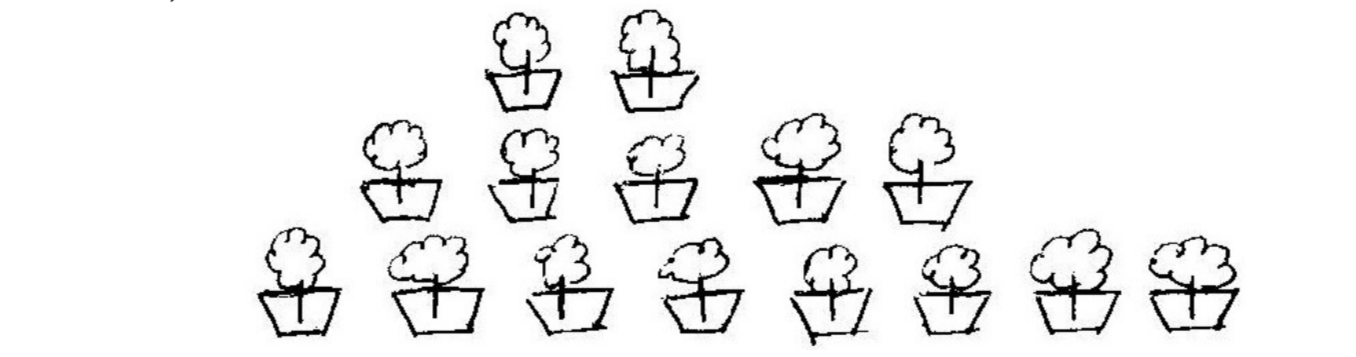
\includegraphics[width=\columnwidth]{figs/Plant.png}
			\caption{Plants}
			\label{fig:Plants}
		\end{figure}
		Based on the above, answer the following questions :
		\begin{enumerate}[label=(\roman*)]
			\item How many pots were placed in the $7^{th}$ row ?
				\begin{enumerate}[label=\Alph*]
					\item $20$
					\item $23$
					\item $77$
					\item $29$
				\end{enumerate}
			\item If Roshini wants to place $100$ pots in total, then total number of rows formed in the arrangement will be ?
				\begin{enumerate}[label=\Alph*]
					\item $8$
					\item $9$
					\item $10$
					\item $12$
				\end{enumerate}
			\item How many pots are placed in the last row ?
				\begin{enumerate}[label=\Alph*]
					\item $20$
					\item $23$
					\item $26$
					\item $29$
				\end{enumerate}
			\item If Roshini ha sufficient space for $12$ rows, then how many total number of pots are placed by her wih the same arrangement ?
				\begin{enumerate}[label=\Alph*]
					\item $222$
					\item $155$
					\item $187$
					\item $313$
				\end{enumerate}
		\end{enumerate} 

	\item Find the LCM and HCF of two numbers $26$ and $91$ by the method of prime factorization.
	\item For two numbers $x$ and $y$, if $xy = 1344$ and HCF $(x,y) = 8$, then find LCM$(x, y)$.
	\item Find the HCF of $96$ and $404$ by prime factorisation.
	\item Express $792$ as the product of its prime factors.
	\item The sum of the first $4$ terms of an A.P. is zero and its $4^{th}$ term is $2$. Find the A.P.
	\item If the sum of the first $n$ terms of an A.P. is given by $S_n = 4n - n^2$, then find its $n^{th}$ term. Hence, find the $25^{th}$ term and the sum if the first 25 terms of this A.P.
	\item If $\alpha$ and $\beta$ are the zeroes of the quadratic polynomial $f(x) = x^{2} - x - 4$, find the value of $\frac{1}{\alpha} + \frac{1}{\beta} - {\alpha \beta}$.
	\item If one zero of the quadratic polynomial $x^{2} +  3x + k$ is $2$, then find the value of $k$.
	\item Find the mean of first $10$ composite numbers.
	\item If $S_n$ denotes the sum of first $n$ terms of an A.P., prove that $S_{12} = 3(S_8 - S_4)$.
	\item After how many decimal places will the decimal expansion of the rational number $\frac{14587}{1250}$ terminate ?			
	\item State giving reason whether $5\times 7\times 11 +11$ is a composite number or a prime number.
	\item If the $6^{th}$ and $14^{th}$ terms of an A.P. are 29 and 69 respectively, then find the $10^{th}$ term of the A.P.
	\item If the first three consecutive terms of an A.P. are $3y-1, 3y+5$ and $5y+1$ find the value of y. 
\end{enumerate}
